\documentclass[]{article}
\usepackage{lmodern}
\usepackage{amssymb,amsmath}
\usepackage{ifxetex,ifluatex}
\usepackage{fixltx2e} % provides \textsubscript
\ifnum 0\ifxetex 1\fi\ifluatex 1\fi=0 % if pdftex
  \usepackage[T1]{fontenc}
  \usepackage[utf8]{inputenc}
\else % if luatex or xelatex
  \ifxetex
    \usepackage{mathspec}
  \else
    \usepackage{fontspec}
  \fi
  \defaultfontfeatures{Ligatures=TeX,Scale=MatchLowercase}
\fi
% use upquote if available, for straight quotes in verbatim environments
\IfFileExists{upquote.sty}{\usepackage{upquote}}{}
% use microtype if available
\IfFileExists{microtype.sty}{%
\usepackage{microtype}
\UseMicrotypeSet[protrusion]{basicmath} % disable protrusion for tt fonts
}{}
\usepackage[margin=1in]{geometry}
\usepackage{hyperref}
\hypersetup{unicode=true,
            pdftitle={Application to 2016 Election Data},
            pdfborder={0 0 0},
            breaklinks=true}
\urlstyle{same}  % don't use monospace font for urls
\usepackage{color}
\usepackage{fancyvrb}
\newcommand{\VerbBar}{|}
\newcommand{\VERB}{\Verb[commandchars=\\\{\}]}
\DefineVerbatimEnvironment{Highlighting}{Verbatim}{commandchars=\\\{\}}
% Add ',fontsize=\small' for more characters per line
\usepackage{framed}
\definecolor{shadecolor}{RGB}{248,248,248}
\newenvironment{Shaded}{\begin{snugshade}}{\end{snugshade}}
\newcommand{\AlertTok}[1]{\textcolor[rgb]{0.94,0.16,0.16}{#1}}
\newcommand{\AnnotationTok}[1]{\textcolor[rgb]{0.56,0.35,0.01}{\textbf{\textit{#1}}}}
\newcommand{\AttributeTok}[1]{\textcolor[rgb]{0.77,0.63,0.00}{#1}}
\newcommand{\BaseNTok}[1]{\textcolor[rgb]{0.00,0.00,0.81}{#1}}
\newcommand{\BuiltInTok}[1]{#1}
\newcommand{\CharTok}[1]{\textcolor[rgb]{0.31,0.60,0.02}{#1}}
\newcommand{\CommentTok}[1]{\textcolor[rgb]{0.56,0.35,0.01}{\textit{#1}}}
\newcommand{\CommentVarTok}[1]{\textcolor[rgb]{0.56,0.35,0.01}{\textbf{\textit{#1}}}}
\newcommand{\ConstantTok}[1]{\textcolor[rgb]{0.00,0.00,0.00}{#1}}
\newcommand{\ControlFlowTok}[1]{\textcolor[rgb]{0.13,0.29,0.53}{\textbf{#1}}}
\newcommand{\DataTypeTok}[1]{\textcolor[rgb]{0.13,0.29,0.53}{#1}}
\newcommand{\DecValTok}[1]{\textcolor[rgb]{0.00,0.00,0.81}{#1}}
\newcommand{\DocumentationTok}[1]{\textcolor[rgb]{0.56,0.35,0.01}{\textbf{\textit{#1}}}}
\newcommand{\ErrorTok}[1]{\textcolor[rgb]{0.64,0.00,0.00}{\textbf{#1}}}
\newcommand{\ExtensionTok}[1]{#1}
\newcommand{\FloatTok}[1]{\textcolor[rgb]{0.00,0.00,0.81}{#1}}
\newcommand{\FunctionTok}[1]{\textcolor[rgb]{0.00,0.00,0.00}{#1}}
\newcommand{\ImportTok}[1]{#1}
\newcommand{\InformationTok}[1]{\textcolor[rgb]{0.56,0.35,0.01}{\textbf{\textit{#1}}}}
\newcommand{\KeywordTok}[1]{\textcolor[rgb]{0.13,0.29,0.53}{\textbf{#1}}}
\newcommand{\NormalTok}[1]{#1}
\newcommand{\OperatorTok}[1]{\textcolor[rgb]{0.81,0.36,0.00}{\textbf{#1}}}
\newcommand{\OtherTok}[1]{\textcolor[rgb]{0.56,0.35,0.01}{#1}}
\newcommand{\PreprocessorTok}[1]{\textcolor[rgb]{0.56,0.35,0.01}{\textit{#1}}}
\newcommand{\RegionMarkerTok}[1]{#1}
\newcommand{\SpecialCharTok}[1]{\textcolor[rgb]{0.00,0.00,0.00}{#1}}
\newcommand{\SpecialStringTok}[1]{\textcolor[rgb]{0.31,0.60,0.02}{#1}}
\newcommand{\StringTok}[1]{\textcolor[rgb]{0.31,0.60,0.02}{#1}}
\newcommand{\VariableTok}[1]{\textcolor[rgb]{0.00,0.00,0.00}{#1}}
\newcommand{\VerbatimStringTok}[1]{\textcolor[rgb]{0.31,0.60,0.02}{#1}}
\newcommand{\WarningTok}[1]{\textcolor[rgb]{0.56,0.35,0.01}{\textbf{\textit{#1}}}}
\usepackage{graphicx,grffile}
\makeatletter
\def\maxwidth{\ifdim\Gin@nat@width>\linewidth\linewidth\else\Gin@nat@width\fi}
\def\maxheight{\ifdim\Gin@nat@height>\textheight\textheight\else\Gin@nat@height\fi}
\makeatother
% Scale images if necessary, so that they will not overflow the page
% margins by default, and it is still possible to overwrite the defaults
% using explicit options in \includegraphics[width, height, ...]{}
\setkeys{Gin}{width=\maxwidth,height=\maxheight,keepaspectratio}
\IfFileExists{parskip.sty}{%
\usepackage{parskip}
}{% else
\setlength{\parindent}{0pt}
\setlength{\parskip}{6pt plus 2pt minus 1pt}
}
\setlength{\emergencystretch}{3em}  % prevent overfull lines
\providecommand{\tightlist}{%
  \setlength{\itemsep}{0pt}\setlength{\parskip}{0pt}}
\setcounter{secnumdepth}{0}
% Redefines (sub)paragraphs to behave more like sections
\ifx\paragraph\undefined\else
\let\oldparagraph\paragraph
\renewcommand{\paragraph}[1]{\oldparagraph{#1}\mbox{}}
\fi
\ifx\subparagraph\undefined\else
\let\oldsubparagraph\subparagraph
\renewcommand{\subparagraph}[1]{\oldsubparagraph{#1}\mbox{}}
\fi

%%% Use protect on footnotes to avoid problems with footnotes in titles
\let\rmarkdownfootnote\footnote%
\def\footnote{\protect\rmarkdownfootnote}

%%% Change title format to be more compact
\usepackage{titling}

% Create subtitle command for use in maketitle
\providecommand{\subtitle}[1]{
  \posttitle{
    \begin{center}\large#1\end{center}
    }
}

\setlength{\droptitle}{-2em}

  \title{Application to 2016 Election Data}
    \pretitle{\vspace{\droptitle}\centering\huge}
  \posttitle{\par}
    \author{}
    \preauthor{}\postauthor{}
    \date{}
    \predate{}\postdate{}
  
\usepackage{booktabs}
\usepackage{longtable}
\usepackage{array}
\usepackage{multirow}
\usepackage{wrapfig}
\usepackage{float}
\usepackage{colortbl}
\usepackage{pdflscape}
\usepackage{tabu}
\usepackage{threeparttable}
\usepackage{threeparttablex}
\usepackage[normalem]{ulem}
\usepackage{makecell}
\usepackage{xcolor}

\usepackage{stackengine}
\usepackage{rotating}

\begin{document}
\maketitle

\begin{Shaded}
\begin{Highlighting}[]
\NormalTok{## Erin's path}
\NormalTok{path_data =}\StringTok{ "~/Dropbox/Documents/2019__2020/work/kpop/2016_reweighting_example/data/"}
\CommentTok{#Ciara's }
\CommentTok{#path_data = "../data/"}
\NormalTok{path_data =}\StringTok{ "/Users/Ciara/Dropbox/kpop/2016_reweighting_example/data/"}
\end{Highlighting}
\end{Shaded}

\begin{Shaded}
\begin{Highlighting}[]
\NormalTok{vote_contrast <-}\StringTok{ }\KeywordTok{quote}\NormalTok{((recode_vote_2016Democrat }\OperatorTok{-}\StringTok{ }\NormalTok{recode_vote_2016Republican) }\OperatorTok{/}
\StringTok{                           }\NormalTok{(recode_vote_2016Democrat }\OperatorTok{+}\StringTok{ }\NormalTok{recode_vote_2016Republican))}

\NormalTok{### Function for creating targets from auxiliary information and formula}
\NormalTok{create_targets <-}\StringTok{ }\ControlFlowTok{function}\NormalTok{ (target_design, target_formula) \{}
\NormalTok{    target_mf <-}\StringTok{ }\KeywordTok{model.frame}\NormalTok{(target_formula, }\KeywordTok{model.frame}\NormalTok{(target_design))}
\NormalTok{    target_mm <-}\StringTok{ }\KeywordTok{model.matrix}\NormalTok{(target_formula, target_mf)}
\NormalTok{    wts <-}\StringTok{ }\KeywordTok{weights}\NormalTok{(target_design)}
    \KeywordTok{colSums}\NormalTok{(target_mm }\OperatorTok{*}\StringTok{ }\NormalTok{wts) }\OperatorTok{/}\StringTok{ }\KeywordTok{sum}\NormalTok{(wts)}
\NormalTok{\}}
\end{Highlighting}
\end{Shaded}

\hypertarget{load-data}{%
\subsection{Load Data}\label{load-data}}

\begin{Shaded}
\begin{Highlighting}[]
\NormalTok{## SURVEY DATA (PEW)}
\NormalTok{### Load}
\NormalTok{pew <-}\StringTok{ }\KeywordTok{readRDS}\NormalTok{(}\KeywordTok{paste0}\NormalTok{(path_data, }\StringTok{"pew.rds"}\NormalTok{))}

\NormalTok{## AUXILIARY INFORMATION (CCES)}
\NormalTok{### Load}
\NormalTok{cces <-}\StringTok{ }\KeywordTok{readRDS}\NormalTok{(}\KeywordTok{paste0}\NormalTok{(path_data, }\StringTok{"cces.rds"}\NormalTok{))}
\NormalTok{### Drop invalid cases}
\NormalTok{cces <-}\StringTok{ }\NormalTok{cces }\OperatorTok
\StringTok{    }\KeywordTok{filter}\NormalTok{((CC16_}\DecValTok{401} \OperatorTok{==}\StringTok{ "I definitely voted in the General Election."}\NormalTok{) }\OperatorTok{&}
\StringTok{               }\OperatorTok{!}\KeywordTok{is.na}\NormalTok{(commonweight_vv_post))}

\NormalTok{## make recode_educ_white column}
\NormalTok{cces <-}\StringTok{ }\NormalTok{cces }\OperatorTok
\StringTok{  }\KeywordTok{mutate}\NormalTok{(}\DataTypeTok{recode_educ_white =} 
           \KeywordTok{factor}\NormalTok{(}\KeywordTok{case_when}\NormalTok{(recode_race }\OperatorTok{==}\StringTok{ "White"} \OperatorTok{~}\StringTok{ }\KeywordTok{as.character}\NormalTok{(recode_educ),}
                            \OtherTok{TRUE} \OperatorTok{~}\StringTok{ "No Split"}\NormalTok{), }
                  \DataTypeTok{levels =} \KeywordTok{c}\NormalTok{(}\KeywordTok{levels}\NormalTok{(cces}\OperatorTok{$}\NormalTok{recode_educ), }\StringTok{"No Split"}\NormalTok{)),}
         \DataTypeTok{commonweight_vv_post =}\NormalTok{ commonweight_vv_post }\OperatorTok{/}\StringTok{ }\KeywordTok{mean}\NormalTok{(commonweight_vv_post))}



\NormalTok{pew <-}\StringTok{ }\NormalTok{pew }\OperatorTok
\StringTok{  }\KeywordTok{mutate}\NormalTok{(}\DataTypeTok{recode_educ_white =} 
           \KeywordTok{factor}\NormalTok{(}\KeywordTok{case_when}\NormalTok{(recode_race }\OperatorTok{==}\StringTok{ "White"} \OperatorTok{~}\StringTok{ }\KeywordTok{as.character}\NormalTok{(recode_educ),}
                            \OtherTok{TRUE} \OperatorTok{~}\StringTok{ "No Split"}\NormalTok{), }
                  \DataTypeTok{levels =} \KeywordTok{c}\NormalTok{(}\KeywordTok{levels}\NormalTok{(pew}\OperatorTok{$}\NormalTok{recode_educ), }\StringTok{"No Split"}\NormalTok{)))}

\NormalTok{### Actual results}
\NormalTok{pres <-}\StringTok{ }\KeywordTok{readRDS}\NormalTok{(}\KeywordTok{paste0}\NormalTok{(path_data, }\StringTok{"election.rds"}\NormalTok{))}

\NormalTok{natl_margin <-}\StringTok{ }\NormalTok{pres }\OperatorTok
\StringTok{    }\KeywordTok{summarise}\NormalTok{(}\DataTypeTok{margin =}\NormalTok{ (}\KeywordTok{sum}\NormalTok{(demtotal) }\OperatorTok{-}\StringTok{ }\KeywordTok{sum}\NormalTok{(reptotal)) }\OperatorTok{/}
\StringTok{                  }\NormalTok{(}\KeywordTok{sum}\NormalTok{(demtotal) }\OperatorTok{+}\StringTok{ }\KeywordTok{sum}\NormalTok{(reptotal))) }\OperatorTok
\StringTok{    }\KeywordTok{as.numeric}\NormalTok{()}
\NormalTok{natl_margin}
\end{Highlighting}
\end{Shaded}

\begin{verbatim}
## [1] 0.02325013
\end{verbatim}

\begin{Shaded}
\begin{Highlighting}[]
\NormalTok{formula_rake_demos_noeduc <-}\StringTok{ }\ErrorTok{~}\NormalTok{recode_age_bucket }\OperatorTok{+}\StringTok{ }\NormalTok{recode_female }\OperatorTok{+}\StringTok{ }
\StringTok{    }\NormalTok{recode_race }\OperatorTok{+}\StringTok{ }\NormalTok{recode_region }\OperatorTok{+}\StringTok{ }\NormalTok{recode_pid_3way}
\NormalTok{formula_rake_demos_weduc <-}\StringTok{ }\ErrorTok{~}\NormalTok{recode_age_bucket }\OperatorTok{+}\StringTok{ }\NormalTok{recode_female }\OperatorTok{+}\StringTok{ }
\StringTok{  }\NormalTok{recode_race }\OperatorTok{+}\StringTok{ }\NormalTok{recode_region }\OperatorTok{+}\StringTok{ }\NormalTok{recode_educ }\OperatorTok{+}\StringTok{ }\NormalTok{recode_pid_3way}
\NormalTok{formula_ps <-}\StringTok{ }\ErrorTok{~}\NormalTok{recode_age_3way }\OperatorTok{+}\StringTok{ }\NormalTok{recode_female }\OperatorTok{+}\StringTok{ }\NormalTok{recode_race }\OperatorTok{+}
\StringTok{    }\NormalTok{recode_region }\OperatorTok{+}\StringTok{ }\NormalTok{recode_educ_3way }\OperatorTok{+}\StringTok{ }\NormalTok{recode_pid_3way}
\NormalTok{formula_retrospective <-}\StringTok{ }\ErrorTok{~}\NormalTok{recode_age_bucket}\OperatorTok{:}\NormalTok{recode_pid_3way }\OperatorTok{+}\StringTok{ }
\StringTok{  }\NormalTok{recode_female}\OperatorTok{:}\NormalTok{recode_pid_3way}\OperatorTok{+}
\StringTok{    }\NormalTok{recode_race_educ_reg}\OperatorTok{:}\NormalTok{recode_pid_3way}
\end{Highlighting}
\end{Shaded}

\begin{Shaded}
\begin{Highlighting}[]
\NormalTok{## Find Missing Strata}
\NormalTok{## Make "strata" variable in CCES and Pew}
\NormalTok{cces <-}\StringTok{ }\KeywordTok{bind_cols}\NormalTok{(cces, cces }\OperatorTok\StringTok{ }
\StringTok{                    }\KeywordTok{unite}\NormalTok{(}\StringTok{"strata"}\NormalTok{, }\KeywordTok{all.vars}\NormalTok{(formula_ps), }\DataTypeTok{remove =} \OtherTok{FALSE}\NormalTok{) }\OperatorTok
\StringTok{                    }\KeywordTok{unite}\NormalTok{(}\StringTok{"strata_wage"}\NormalTok{, }\KeywordTok{c}\NormalTok{(}\KeywordTok{all.vars}\NormalTok{(formula_ps), }\StringTok{"recode_age"}\NormalTok{), }
                          \DataTypeTok{remove =} \OtherTok{FALSE}\NormalTok{) }\OperatorTok
\StringTok{                    }\KeywordTok{select}\NormalTok{(strata, strata_wage))}

\NormalTok{pew <-}\StringTok{ }\KeywordTok{bind_cols}\NormalTok{(pew, pew }\OperatorTok\StringTok{ }
\StringTok{                   }\KeywordTok{unite}\NormalTok{(}\StringTok{"strata"}\NormalTok{, }\KeywordTok{all.vars}\NormalTok{(formula_ps), }\DataTypeTok{remove =} \OtherTok{FALSE}\NormalTok{) }\OperatorTok
\StringTok{                   }\KeywordTok{unite}\NormalTok{(}\StringTok{"strata_wage"}\NormalTok{, }\KeywordTok{c}\NormalTok{(}\KeywordTok{all.vars}\NormalTok{(formula_ps), }\StringTok{"recode_age"}\NormalTok{), }
                         \DataTypeTok{remove =} \OtherTok{FALSE}\NormalTok{) }\OperatorTok
\StringTok{                   }\KeywordTok{select}\NormalTok{(strata, strata_wage))}


\NormalTok{missing_strata <-}\StringTok{ }\KeywordTok{unique}\NormalTok{(cces}\OperatorTok{$}\NormalTok{strata)[}\OperatorTok{!}\NormalTok{(}\KeywordTok{unique}\NormalTok{(cces}\OperatorTok{$}\NormalTok{strata) }\OperatorTok\StringTok{ }\KeywordTok{unique}\NormalTok{(pew}\OperatorTok{$}\NormalTok{strata))]}

\NormalTok{## recode missing age}

\NormalTok{#####XXXXXX issue here: how to recode age and whether to recode age buckets}
\CommentTok{#pew$recode_age[is.na(pew$recode_age)] <- mean(pew$recode_age, na.rm = TRUE)}
\NormalTok{pew}\OperatorTok{$}\NormalTok{recode_age[}\KeywordTok{is.na}\NormalTok{(pew}\OperatorTok{$}\NormalTok{recode_age)] <-}\StringTok{ }\KeywordTok{mean}\NormalTok{(cces}\OperatorTok{$}\NormalTok{recode_age, }\DataTypeTok{na.rm =} \OtherTok{TRUE}\NormalTok{)}
\NormalTok{cces}\OperatorTok{$}\NormalTok{recode_age[}\KeywordTok{is.na}\NormalTok{(cces}\OperatorTok{$}\NormalTok{recode_age)] <-}\StringTok{ }\KeywordTok{mean}\NormalTok{(cces}\OperatorTok{$}\NormalTok{recode_age, }\DataTypeTok{na.rm =} \OtherTok{TRUE}\NormalTok{)}

\NormalTok{## For Pew, since there are no design weights, assume SRS}
\NormalTok{pew_srs <-}\StringTok{ }\KeywordTok{svydesign}\NormalTok{(}\DataTypeTok{ids =} \OperatorTok{~}\DecValTok{1}\NormalTok{, }\DataTypeTok{data =}\NormalTok{ pew)}
\NormalTok{cces_awt <-}\StringTok{ }\KeywordTok{svydesign}\NormalTok{(}\DataTypeTok{ids =} \OperatorTok{~}\DecValTok{1}\NormalTok{, }\DataTypeTok{weights =} \OperatorTok{~}\NormalTok{commonweight_vv_post, }\DataTypeTok{data =}\NormalTok{ cces)}
\end{Highlighting}
\end{Shaded}

\begin{Shaded}
\begin{Highlighting}[]
\NormalTok{### Population targets}
\NormalTok{targets_rake_demos_noeduc <-}\StringTok{ }\KeywordTok{create_targets}\NormalTok{(cces_awt, formula_rake_demos_noeduc)}
\NormalTok{targets_rake_demos_weduc <-}\StringTok{ }\KeywordTok{create_targets}\NormalTok{(cces_awt, formula_rake_demos_weduc)}
\NormalTok{targets_retrospective <-}\StringTok{ }\KeywordTok{create_targets}\NormalTok{(cces_awt, formula_retrospective)}
\end{Highlighting}
\end{Shaded}

\begin{Shaded}
\begin{Highlighting}[]
\NormalTok{## Raking on demographics, excluding education}
\NormalTok{rake_demos_noeduc <-}\StringTok{ }\KeywordTok{calibrate}\NormalTok{(}\DataTypeTok{design =}\NormalTok{ pew_srs,}
                       \DataTypeTok{formula =}\NormalTok{ formula_rake_demos_noeduc,}
                       \DataTypeTok{population =}\NormalTok{ targets_rake_demos_noeduc,}
                       \DataTypeTok{calfun =} \StringTok{"raking"}\NormalTok{)}

\NormalTok{rake_demos_noeduc <-}\StringTok{ }\KeywordTok{svydesign}\NormalTok{(}\OperatorTok{~}\DecValTok{1}\NormalTok{, }\DataTypeTok{data =}\NormalTok{ pew, }\DataTypeTok{weights =} \KeywordTok{weights}\NormalTok{(rake_demos_noeduc))}

\NormalTok{## Raking on demographics, including education}
\NormalTok{rake_demos_weduc <-}\StringTok{ }\KeywordTok{calibrate}\NormalTok{(}\DataTypeTok{design =}\NormalTok{ pew_srs,}
                              \DataTypeTok{formula =}\NormalTok{ formula_rake_demos_weduc,}
                              \DataTypeTok{population =}\NormalTok{ targets_rake_demos_weduc,}
                              \DataTypeTok{calfun =} \StringTok{"raking"}\NormalTok{)}

\NormalTok{rake_demos_weduc <-}\StringTok{ }\KeywordTok{svydesign}\NormalTok{(}\OperatorTok{~}\DecValTok{1}\NormalTok{, }\DataTypeTok{data =}\NormalTok{ pew, }\DataTypeTok{weights =} \KeywordTok{weights}\NormalTok{(rake_demos_weduc))}

\NormalTok{## Post-stratification}
\NormalTok{targets_ps <-}\StringTok{ }\KeywordTok{svytable}\NormalTok{(}\DataTypeTok{formula =} \OperatorTok{~}\NormalTok{strata, }
                       \DataTypeTok{design =} \KeywordTok{subset}\NormalTok{(cces_awt, }\OperatorTok{!}\NormalTok{(strata }\OperatorTok\StringTok{ }\NormalTok{missing_strata)))}

\NormalTok{post_stratification <-}\StringTok{ }\KeywordTok{postStratify}\NormalTok{(}\DataTypeTok{design =}\NormalTok{ pew_srs,}
                         \DataTypeTok{strata =} \OperatorTok{~}\NormalTok{strata,}
                         \DataTypeTok{population =}\NormalTok{ targets_ps)}

\NormalTok{post_stratification <-}\StringTok{ }\KeywordTok{svydesign}\NormalTok{(}\OperatorTok{~}\DecValTok{1}\NormalTok{, }\DataTypeTok{data =}\NormalTok{ pew, }
                                 \DataTypeTok{weights =} \KeywordTok{weights}\NormalTok{(post_stratification))}

\NormalTok{## Retrospective weighting scheme}
\CommentTok{#failed to converge? XX}
\NormalTok{rake_retrospective <-}\StringTok{ }\KeywordTok{calibrate}\NormalTok{(}\DataTypeTok{design =}\NormalTok{ pew_srs,}
                              \DataTypeTok{formula =}\NormalTok{ formula_retrospective,}
                              \DataTypeTok{population =}\NormalTok{ targets_retrospective,}
                              \DataTypeTok{calfun =} \StringTok{"raking"}\NormalTok{,}
                              \DataTypeTok{force =} \OtherTok{TRUE}\NormalTok{)}
\end{Highlighting}
\end{Shaded}

\begin{verbatim}
## Warning in grake(mm, ww, calfun, bounds = bounds, population =
## population, : Failed to converge: eps=0.00688873036014645 in 51 iterations
\end{verbatim}

\begin{Shaded}
\begin{Highlighting}[]
\NormalTok{rake_retrospective <-}\StringTok{ }\KeywordTok{svydesign}\NormalTok{(}\OperatorTok{~}\DecValTok{1}\NormalTok{, }\DataTypeTok{data =}\NormalTok{ pew, }\DataTypeTok{weights =} \KeywordTok{weights}\NormalTok{(rake_retrospective))}
\end{Highlighting}
\end{Shaded}

\begin{Shaded}
\begin{Highlighting}[]
\NormalTok{kpop_data <-}\StringTok{ }\KeywordTok{rbind}\NormalTok{(pew }\OperatorTok\StringTok{ }\KeywordTok{select}\NormalTok{(recode_age,}
\NormalTok{                                  recode_female,}
\NormalTok{                                  recode_race, }
\NormalTok{                                  recode_region, }
\NormalTok{                                  recode_pid_3way,}
\NormalTok{                                  recode_educ, }
\NormalTok{                                  recode_age_bucket),}
\NormalTok{                   cces }\OperatorTok\StringTok{ }\KeywordTok{select}\NormalTok{(recode_age, }
\NormalTok{                                   recode_female, }
\NormalTok{                                   recode_race, }
\NormalTok{                                   recode_region,}
\NormalTok{                                   recode_pid_3way, }
\NormalTok{                                   recode_educ,}
\NormalTok{                                   recode_age_bucket)) }\OperatorTok
\StringTok{   }\KeywordTok{model.matrix}\NormalTok{(}\KeywordTok{as.formula}\NormalTok{(}\StringTok{"~. - 1"}\NormalTok{), .)}


\NormalTok{kpop_sampled <-}\StringTok{ }\KeywordTok{c}\NormalTok{(}\KeywordTok{rep}\NormalTok{(}\DecValTok{1}\NormalTok{, }\KeywordTok{nrow}\NormalTok{(pew)), }\KeywordTok{rep}\NormalTok{(}\DecValTok{0}\NormalTok{, }\KeywordTok{nrow}\NormalTok{(cces)))}

\NormalTok{kpop_b}\FloatTok{.5}\NormalTok{x <-}\StringTok{ }\KeywordTok{kbal}\NormalTok{(}\DataTypeTok{allx=}\NormalTok{kpop_data,}
                    \DataTypeTok{sampled =}\NormalTok{ kpop_sampled,}
                    \DataTypeTok{b =} \FloatTok{0.5} \OperatorTok{*}\StringTok{ }\KeywordTok{ncol}\NormalTok{(kpop_data),}
                    \DataTypeTok{fullSVD =} \OtherTok{TRUE}\NormalTok{,}
                    \DataTypeTok{meanfirst =} \OtherTok{FALSE}\NormalTok{,}
                    \DataTypeTok{incrementby =} \DecValTok{1}\NormalTok{,}
    \DataTypeTok{population.w =}\NormalTok{ cces}\OperatorTok{$}\NormalTok{commonweight_vv_post }\OperatorTok{/}\KeywordTok{mean}\NormalTok{(cces}\OperatorTok{$}\NormalTok{commonweight_vv_post),}
                    \DataTypeTok{sampledinpop =} \OtherTok{FALSE}\NormalTok{,}
                    \DataTypeTok{printprogress =} \OtherTok{FALSE}\NormalTok{)}

\NormalTok{kpop_mf_b2x <-}\StringTok{ }\KeywordTok{kbal}\NormalTok{(}\DataTypeTok{allx=}\NormalTok{kpop_data,}
                      \DataTypeTok{sampled =}\NormalTok{ kpop_sampled,}
                      \DataTypeTok{b =} \DecValTok{2} \OperatorTok{*}\StringTok{ }\KeywordTok{ncol}\NormalTok{(kpop_data),}
                      \DataTypeTok{incrementby =} \DecValTok{1}\NormalTok{,}
                      \DataTypeTok{fullSVD =} \OtherTok{TRUE}\NormalTok{,}
                      \DataTypeTok{meanfirst =} \OtherTok{TRUE}\NormalTok{,}
                      \DataTypeTok{ebal.convergence =} \OtherTok{TRUE}\NormalTok{, }
        \DataTypeTok{population.w =}\NormalTok{ cces}\OperatorTok{$}\NormalTok{commonweight_vv_post}\OperatorTok{/}\KeywordTok{mean}\NormalTok{(cces}\OperatorTok{$}\NormalTok{commonweight_vv_post),}
                      \DataTypeTok{sampledinpop =} \OtherTok{FALSE}\NormalTok{,}
                      \DataTypeTok{printprogress =} \OtherTok{FALSE}\NormalTok{)}

\NormalTok{kpop <-}\StringTok{ }\KeywordTok{svydesign}\NormalTok{(}\OperatorTok{~}\DecValTok{1}\NormalTok{, }\DataTypeTok{data =}\NormalTok{ pew, }\DataTypeTok{weights =}\NormalTok{ kpop_b}\FloatTok{.5}\NormalTok{x}\OperatorTok{$}\NormalTok{w[kpop_sampled] )}
\NormalTok{kpop_mf <-}\StringTok{ }\KeywordTok{svydesign}\NormalTok{(}\OperatorTok{~}\DecValTok{1}\NormalTok{, }\DataTypeTok{data =}\NormalTok{ pew, }\DataTypeTok{weights =}\NormalTok{ kpop_mf_b2x}\OperatorTok{$}\NormalTok{w[kpop_sampled])}
\end{Highlighting}
\end{Shaded}

\begin{Shaded}
\begin{Highlighting}[]
\NormalTok{margin_summary <-}\StringTok{ }\KeywordTok{round}\NormalTok{(}\KeywordTok{cbind}\NormalTok{(}\DataTypeTok{cces =} \KeywordTok{svymean}\NormalTok{(formula_rake_demos_weduc, cces_awt),}
                              \DataTypeTok{unweighted =} \KeywordTok{svymean}\NormalTok{(formula_rake_demos_weduc, pew_srs),}
            \DataTypeTok{rake_demos_noeduc =} \KeywordTok{svymean}\NormalTok{(formula_rake_demos_weduc, rake_demos_noeduc),}
            \DataTypeTok{rake_demos_weduc =} \KeywordTok{svymean}\NormalTok{(formula_rake_demos_weduc, rake_demos_weduc),}
            \DataTypeTok{post_stratification =} \KeywordTok{svymean}\NormalTok{(formula_rake_demos_weduc, post_stratification),}
            \DataTypeTok{rake_retrospective =} \KeywordTok{svymean}\NormalTok{(formula_rake_demos_weduc, rake_retrospective),}
            \DataTypeTok{kpop =} \KeywordTok{svymean}\NormalTok{(formula_rake_demos_weduc, kpop),}
            \DataTypeTok{kpop_mf =} \KeywordTok{svymean}\NormalTok{(formula_rake_demos_weduc, kpop_mf)) }\OperatorTok{*}\StringTok{ }\DecValTok{100}\NormalTok{, }\DecValTok{1}\NormalTok{) }\OperatorTok
\StringTok{  }\KeywordTok{data.frame}\NormalTok{() }\OperatorTok
\StringTok{  }\KeywordTok{rownames_to_column}\NormalTok{() }\OperatorTok
\StringTok{  }\KeywordTok{mutate}\NormalTok{(}\DataTypeTok{variable =} \KeywordTok{case_when}\NormalTok{(}\KeywordTok{str_detect}\NormalTok{(rowname, }\StringTok{"age"}\NormalTok{) }\OperatorTok{~}\StringTok{ "4-way Age Bucket"}\NormalTok{,}
                             \KeywordTok{str_detect}\NormalTok{(rowname, }\StringTok{"female"}\NormalTok{) }\OperatorTok{~}\StringTok{ "Gender"}\NormalTok{,}
                             \KeywordTok{str_detect}\NormalTok{(rowname, }\StringTok{"race"}\NormalTok{) }\OperatorTok{~}\StringTok{ "Race/Ethnicity"}\NormalTok{,}
                             \KeywordTok{str_detect}\NormalTok{(rowname, }\StringTok{"region"}\NormalTok{) }\OperatorTok{~}\StringTok{ "Region"}\NormalTok{,}
                             \KeywordTok{str_detect}\NormalTok{(rowname, }\StringTok{"educ"}\NormalTok{) }\OperatorTok{~}\StringTok{ "Education Level"}\NormalTok{,}
                             \KeywordTok{str_detect}\NormalTok{(rowname, }\StringTok{"pid"}\NormalTok{) }\OperatorTok{~}\StringTok{ "Party Identification"}\NormalTok{,}
                             \OtherTok{TRUE} \OperatorTok{~}\StringTok{ "Empty"}\NormalTok{),}
         \DataTypeTok{level =} 
           \KeywordTok{gsub}\NormalTok{(}\StringTok{"recode_|age_bucket|female|race|region|educ|pid_3way"}\NormalTok{, }\StringTok{""}\NormalTok{, rowname)) }\OperatorTok
\StringTok{  }\KeywordTok{select}\NormalTok{(level, }\KeywordTok{everything}\NormalTok{(), }\OperatorTok{-}\NormalTok{rowname, }\OperatorTok{-}\NormalTok{variable)}
\end{Highlighting}
\end{Shaded}

\begin{table}[t]

\caption{\label{tab:margins_table}Marginal distribution, in precentage points, of important demographics under different weighting models.}
\centering
\begin{threeparttable}
\begin{tabular}{>{\raggedright\arraybackslash}p{1.45in}>{\raggedleft\arraybackslash}p{0.45in}>{\raggedleft\arraybackslash}p{0.45in}>{\raggedleft\arraybackslash}p{0.45in}>{\raggedleft\arraybackslash}p{0.45in}>{\raggedleft\arraybackslash}p{0.45in}>{\raggedleft\arraybackslash}p{0.45in}>{\raggedleft\arraybackslash}p{0.45in}>{\raggedleft\arraybackslash}p{0.45in}}
\toprule
 & \belowbaseline[0ex]{\rotatebox{90}{\parbox{1.1in}{\raggedright{Target (CCES)}}}} & \belowbaseline[0ex]{\rotatebox{90}{\parbox{1.1in}{\raggedright{Unweighted Pew}}}} & \belowbaseline[0ex]{\rotatebox{90}{\parbox{1.1in}{\raggedright{Raking:\\Demographics}}}} & \belowbaseline[0ex]{\rotatebox{90}{\parbox{1.1in}{\raggedright{Raking:\\Demographics + Education}}}} & \belowbaseline[0ex]{\rotatebox{90}{\parbox{1.1in}{\raggedright{Post-Stratification}}}} & \belowbaseline[0ex]{\rotatebox{90}{\parbox{1.1in}{\raggedright{Raking:\\Retrospective}}}} & \belowbaseline[0ex]{\rotatebox{90}{\parbox{1.1in}{\raggedright{KPop}}}} & \belowbaseline[0ex]{\rotatebox{90}{\parbox{1.1in}{\raggedright{KPop Mean First}}}}\\
\midrule
\addlinespace[0.5em]
\multicolumn{9}{l}{\textbf{4-way Age Bucket}}\\
\hspace{1em}18 to 35 & 34.8 & 43.7 & 34.8 & 34.8 & 35.4 & 34.8 & 34.4 & 34.8\\
\hspace{1em}36 to 50 & 22.6 & 32.6 & 22.6 & 22.6 & 26.7 & 22.6 & 23.6 & 22.6\\
\hspace{1em}51 to 64 & 28.9 & 21.0 & 28.9 & 28.9 & 29.7 & 28.9 & 29.5 & 28.9\\
\hspace{1em}65+ & 13.7 & 2.7 & 13.7 & 13.7 & 8.3 & 13.7 & 12.5 & 13.7\\
\addlinespace[0.5em]
\multicolumn{9}{l}{\textbf{Gender}}\\
\hspace{1em}Female & 50.8 & 47.3 & 50.8 & 50.8 & 50.8 & 50.8 & 50.8 & 50.8\\
\hspace{1em}Male & 49.2 & 52.7 & 49.2 & 49.2 & 49.2 & 49.2 & 49.2 & 49.2\\
\addlinespace[0.5em]
\multicolumn{9}{l}{\textbf{Race/Ethnicity}}\\
\hspace{1em}Black & 11.8 & 8.9 & 11.8 & 11.8 & 11.5 & 13.4 & 11.7 & 11.8\\
\hspace{1em}Hispanic & 6.5 & 7.6 & 6.5 & 6.5 & 6.2 & 6.5 & 5.9 & 6.5\\
\hspace{1em}Other & 6.8 & 7.1 & 6.8 & 6.8 & 6.5 & 6.8 & 6.2 & 6.8\\
\hspace{1em}White & 74.9 & 76.4 & 74.9 & 74.9 & 75.8 & 73.2 & 76.3 & 74.9\\
\addlinespace[0.5em]
\multicolumn{9}{l}{\textbf{Region}}\\
\hspace{1em}Midwest & 23.4 & 22.3 & 23.4 & 23.4 & 23.2 & 24.7 & 23.6 & 23.4\\
\hspace{1em}Northeast & 19.7 & 18.2 & 19.7 & 19.7 & 19.3 & 19.7 & 19.5 & 19.7\\
\hspace{1em}South & 35.5 & 37.9 & 35.5 & 35.5 & 36.9 & 34.8 & 36.0 & 35.5\\
\hspace{1em}West & 21.4 & 21.6 & 21.4 & 21.4 & 20.6 & 20.8 & 20.8 & 21.4\\
\addlinespace[0.5em]
\multicolumn{9}{l}{\textbf{Education Level}}\\
\hspace{1em}No HS & 6.8 & 1.8 & 1.8 & 6.8 & 2.4 & 3.6 & 1.9 & 6.8\\
\hspace{1em}High school & 30.6 & 19.7 & 21.5 & 30.6 & 28.8 & 29.4 & 31.2 & 30.6\\
\hspace{1em}Some college & 23.0 & 16.7 & 17.7 & 23.0 & 24.5 & 23.0 & 24.4 & 23.0\\
\hspace{1em}2-year & 10.6 & 11.3 & 10.6 & 10.6 & 9.5 & 11.7 & 10.9 & 10.6\\
\hspace{1em}4-year & 18.7 & 28.6 & 26.2 & 18.7 & 22.2 & 20.2 & 20.3 & 18.7\\
\hspace{1em}Post-grad & 10.4 & 21.9 & 22.3 & 10.4 & 12.6 & 12.2 & 11.3 & 10.4\\
\addlinespace[0.5em]
\multicolumn{9}{l}{\textbf{Party Identification}}\\
\hspace{1em}Dem & 38.1 & 34.4 & 38.1 & 38.1 & 38.5 & 38.1 & 37.6 & 38.1\\
\hspace{1em}Ind & 32.5 & 35.2 & 32.5 & 32.5 & 32.5 & 32.5 & 32.8 & 32.5\\
\hspace{1em}Rep & 29.5 & 30.4 & 29.5 & 29.5 & 29.0 & 29.5 & 29.5 & 29.5\\
\bottomrule
\end{tabular}
\begin{tablenotes}
\item \textit{Note: } 
\item Cells present the percentage of the population represented by each variable level.
\end{tablenotes}
\end{threeparttable}
\end{table}

\begin{Shaded}
\begin{Highlighting}[]
\NormalTok{## Total missing strata}
\KeywordTok{sum}\NormalTok{(cces}\OperatorTok{$}\NormalTok{commonweight_vv_post[cces}\OperatorTok{$}\NormalTok{strata }\OperatorTok\StringTok{ }\NormalTok{missing_strata])}\OperatorTok{/}\KeywordTok{sum}\NormalTok{(cces}\OperatorTok{$}\NormalTok{commonweight_vv_post)}
\end{Highlighting}
\end{Shaded}

\begin{verbatim}
## [1] 0.08405765
\end{verbatim}

\begin{Shaded}
\begin{Highlighting}[]
\KeywordTok{round}\NormalTok{(}\KeywordTok{cbind}\NormalTok{(}\DataTypeTok{cces =} \KeywordTok{svymean}\NormalTok{(formula_rake_demos_weduc, cces_awt),}
            \DataTypeTok{not_missing =} \KeywordTok{svymean}\NormalTok{(formula_rake_demos_weduc, }
                                  \KeywordTok{subset}\NormalTok{(cces_awt, }\OperatorTok{!}\NormalTok{(strata }\OperatorTok\StringTok{ }\NormalTok{missing_strata))),}
            \DataTypeTok{missing =} \KeywordTok{svymean}\NormalTok{(formula_rake_demos_weduc, }
                              \KeywordTok{subset}\NormalTok{(cces_awt, (strata }\OperatorTok\StringTok{ }\NormalTok{missing_strata)))) }\OperatorTok{*}\StringTok{ }\DecValTok{100}\NormalTok{, }\DecValTok{1}\NormalTok{) }\OperatorTok
\StringTok{  }\KeywordTok{data.frame}\NormalTok{() }\OperatorTok
\StringTok{  }\KeywordTok{rownames_to_column}\NormalTok{() }\OperatorTok
\StringTok{  }\KeywordTok{mutate}\NormalTok{(}\DataTypeTok{variable =} \KeywordTok{case_when}\NormalTok{(}\KeywordTok{str_detect}\NormalTok{(rowname, }\StringTok{"age"}\NormalTok{) }\OperatorTok{~}\StringTok{ "4-way Age Bucket"}\NormalTok{,}
                             \KeywordTok{str_detect}\NormalTok{(rowname, }\StringTok{"female"}\NormalTok{) }\OperatorTok{~}\StringTok{ "Gender"}\NormalTok{,}
                             \KeywordTok{str_detect}\NormalTok{(rowname, }\StringTok{"race"}\NormalTok{) }\OperatorTok{~}\StringTok{ "Race/Ethnicity"}\NormalTok{,}
                             \KeywordTok{str_detect}\NormalTok{(rowname, }\StringTok{"region"}\NormalTok{) }\OperatorTok{~}\StringTok{ "Region"}\NormalTok{,}
                             \KeywordTok{str_detect}\NormalTok{(rowname, }\StringTok{"educ"}\NormalTok{) }\OperatorTok{~}\StringTok{ "Education Level"}\NormalTok{,}
                             \KeywordTok{str_detect}\NormalTok{(rowname, }\StringTok{"pid"}\NormalTok{) }\OperatorTok{~}\StringTok{ "Party Identification"}\NormalTok{,}
                             \OtherTok{TRUE} \OperatorTok{~}\StringTok{ "Empty"}\NormalTok{),}
         \DataTypeTok{level =} 
           \KeywordTok{gsub}\NormalTok{(}\StringTok{"recode_|age_bucket|female|race|region|educ|pid_3way"}\NormalTok{, }\StringTok{""}\NormalTok{, rowname)) }\OperatorTok
\StringTok{  }\KeywordTok{select}\NormalTok{(level, }\KeywordTok{everything}\NormalTok{(), }\OperatorTok{-}\NormalTok{rowname, }\OperatorTok{-}\NormalTok{variable)}
\end{Highlighting}
\end{Shaded}

\begin{verbatim}
##                   level cces not_missing missing
## 1              18 to 35 34.8        37.6     4.0
## 2              36 to 50 22.6        24.5     2.0
## 3              51 to 64 28.9        29.7    20.6
## 4                   65+ 13.7         8.3    73.4
## 5                Female 50.8        50.8    51.5
## 6                  Male 49.2        49.2    48.5
## 7                 Black 11.8        11.5    14.9
## 8              Hispanic  6.5         6.2    10.1
## 9                 Other  6.8         6.5    10.3
## 10                White 74.9        75.8    64.8
## 11              Midwest 23.4        23.2    25.5
## 12            Northeast 19.7        19.3    24.4
## 13                South 35.5        36.9    19.9
## 14                 West 21.4        20.6    30.2
## 15                No HS  6.8         6.2    13.2
## 16 High school graduate 30.6        30.3    32.9
## 17         Some college 23.0        23.5    17.6
## 18               2-year 10.6        10.8     8.6
## 19               4-year 18.7        19.0    15.0
## 20            Post-grad 10.4        10.1    12.8
## 21                  Dem 38.1        38.5    33.1
## 22                  Ind 32.5        32.5    32.0
## 23                  Rep 29.5        29.0    34.9
\end{verbatim}

\begin{Shaded}
\begin{Highlighting}[]
\NormalTok{margin_summary_educ <-}\StringTok{ }\KeywordTok{round}\NormalTok{(}\KeywordTok{cbind}\NormalTok{(}\DataTypeTok{cces =} \KeywordTok{svymean}\NormalTok{(}\OperatorTok{~}\NormalTok{recode_educ_white, cces_awt),}
                              \DataTypeTok{unweighted =} \KeywordTok{svymean}\NormalTok{(}\OperatorTok{~}\NormalTok{recode_educ_white, pew_srs),}
            \DataTypeTok{rake_demos_noeduc =} \KeywordTok{svymean}\NormalTok{(}\OperatorTok{~}\NormalTok{recode_educ_white, rake_demos_noeduc),}
            \DataTypeTok{rake_demos_weduc =} \KeywordTok{svymean}\NormalTok{(}\OperatorTok{~}\NormalTok{recode_educ_white, rake_demos_weduc),}
            \DataTypeTok{post_stratification =} \KeywordTok{svymean}\NormalTok{(}\OperatorTok{~}\NormalTok{recode_educ_white, post_stratification),}
            \DataTypeTok{rake_retrospective =} \KeywordTok{svymean}\NormalTok{(}\OperatorTok{~}\NormalTok{recode_educ_white, rake_retrospective),}
            \DataTypeTok{kpop =} \KeywordTok{svymean}\NormalTok{(}\OperatorTok{~}\NormalTok{recode_educ_white, kpop),}
            \DataTypeTok{kpop_mf =} \KeywordTok{svymean}\NormalTok{(}\OperatorTok{~}\NormalTok{recode_educ_white, kpop_mf)) }\OperatorTok{*}\StringTok{ }\DecValTok{100}\NormalTok{, }\DecValTok{1}\NormalTok{) }\OperatorTok
\StringTok{  }\KeywordTok{data.frame}\NormalTok{() }\OperatorTok
\StringTok{  }\KeywordTok{rownames_to_column}\NormalTok{() }\OperatorTok
\StringTok{  }\KeywordTok{mutate}\NormalTok{(}\DataTypeTok{variable =} \KeywordTok{case_when}\NormalTok{(}\KeywordTok{str_detect}\NormalTok{(rowname, }\StringTok{"age"}\NormalTok{) }\OperatorTok{~}\StringTok{ "4-way Age Bucket"}\NormalTok{,}
                             \KeywordTok{str_detect}\NormalTok{(rowname, }\StringTok{"female"}\NormalTok{) }\OperatorTok{~}\StringTok{ "Gender"}\NormalTok{,}
                             \KeywordTok{str_detect}\NormalTok{(rowname, }\StringTok{"race"}\NormalTok{) }\OperatorTok{~}\StringTok{ "Race/Ethnicity"}\NormalTok{,}
                             \KeywordTok{str_detect}\NormalTok{(rowname, }\StringTok{"region"}\NormalTok{) }\OperatorTok{~}\StringTok{ "Region"}\NormalTok{,}
                             \KeywordTok{str_detect}\NormalTok{(rowname, }\StringTok{"educ"}\NormalTok{) }\OperatorTok{~}\StringTok{ "Education Level"}\NormalTok{,}
                             \KeywordTok{str_detect}\NormalTok{(rowname, }\StringTok{"pid"}\NormalTok{) }\OperatorTok{~}\StringTok{ "Party Identification"}\NormalTok{,}
                             \OtherTok{TRUE} \OperatorTok{~}\StringTok{ "Empty"}\NormalTok{),}
         \DataTypeTok{level =} 
           \KeywordTok{gsub}\NormalTok{(}\StringTok{"recode_|age_bucket|female|race|region|educ|pid_3way|educ_3way|_white"}\NormalTok{, }
                \StringTok{""}\NormalTok{, rowname)) }\OperatorTok
\StringTok{  }\KeywordTok{select}\NormalTok{(level, }\KeywordTok{everything}\NormalTok{(), }\OperatorTok{-}\NormalTok{rowname, }\OperatorTok{-}\NormalTok{variable)}
\end{Highlighting}
\end{Shaded}

\begin{verbatim}
## Warning: funs() is soft deprecated as of dplyr 0.8.0
## Please use a list of either functions or lambdas: 
## 
##   # Simple named list: 
##   list(mean = mean, median = median)
## 
##   # Auto named with `tibble::lst()`: 
##   tibble::lst(mean, median)
## 
##   # Using lambdas
##   list(~ mean(., trim = .2), ~ median(., na.rm = TRUE))
## This warning is displayed once per session.
\end{verbatim}

\begin{table}[t]

\caption{\label{tab:margins_table_educ}Marginal distribution of education level for white voters under different weighting models.}
\centering
\begin{threeparttable}
\begin{tabular}{>{\raggedright\arraybackslash}p{1.68in}>{\raggedleft\arraybackslash}p{0.45in}>{\raggedleft\arraybackslash}p{0.45in}>{\raggedleft\arraybackslash}p{0.45in}>{\raggedleft\arraybackslash}p{0.45in}>{\raggedleft\arraybackslash}p{0.45in}>{\raggedleft\arraybackslash}p{0.45in}>{\raggedleft\arraybackslash}p{0.45in}>{\raggedleft\arraybackslash}p{0.45in}}
\toprule
 & \belowbaseline[0ex]{\rotatebox{90}{\parbox{1.1in}{\raggedright{Target (CCES)}}}} & \belowbaseline[0ex]{\rotatebox{90}{\parbox{1.1in}{\raggedright{Unweighted Pew}}}} & \belowbaseline[0ex]{\rotatebox{90}{\parbox{1.1in}{\raggedright{Raking:\\Demographics}}}} & \belowbaseline[0ex]{\rotatebox{90}{\parbox{1.1in}{\raggedright{Raking:\\Demographics + Education}}}} & \belowbaseline[0ex]{\rotatebox{90}{\parbox{1.1in}{\raggedright{Post-Stratification}}}} & \belowbaseline[0ex]{\rotatebox{90}{\parbox{1.1in}{\raggedright{Raking:\\Retrospective}}}} & \belowbaseline[0ex]{\rotatebox{90}{\parbox{1.1in}{\raggedright{KPop}}}} & \belowbaseline[0ex]{\rotatebox{90}{\parbox{1.1in}{\raggedright{KPop Mean First}}}}\\
\midrule
\addlinespace[0.5em]
\multicolumn{9}{l}{\textbf{Education Level for White Voters}}\\
\hspace{1em}No HS & 4.6 & 1.1 & 1.1 & 4.5 & 1.8 & 3.0 & 1.2 & 4.8\\
\hspace{1em}High school & 22.6 & 14.6 & 15.5 & 22.9 & 23.1 & 22.6 & 23.6 & 21.9\\
\hspace{1em}Some college & 16.9 & 11.5 & 12.1 & 16.3 & 19.5 & 16.9 & 18.3 & 17.7\\
\hspace{1em}2-year & 7.8 & 8.3 & 7.0 & 7.3 & 6.1 & 7.8 & 7.7 & 7.2\\
\hspace{1em}4-year & 14.8 & 23.0 & 20.7 & 15.2 & 17.1 & 14.8 & 16.3 & 14.8\\
\hspace{1em}Post-grad & 8.3 & 18.0 & 18.5 & 8.8 & 8.2 & 8.3 & 9.1 & 8.4\\
\addlinespace[0.5em]
\multicolumn{9}{l}{\textbf{Error}}\\
\hspace{1em}Mean Absolute Error & -- & 6.6 & 5.8 & 0.4 & 1.6 & 0.1 & 1.2 & 0.5\\
\bottomrule
\end{tabular}
\begin{tablenotes}
\item \textit{Note: } 
\item Cells present the percentage of the population represented by each variable level.  Mean absolute error is the absoluate error in each cell, relative to the target (CCES), weighted by the edcuation level's proportion among white voters in the target population.
\end{tablenotes}
\end{threeparttable}
\end{table}

\begin{Shaded}
\begin{Highlighting}[]
\NormalTok{target_margin <-}\StringTok{ }\KeywordTok{svycontrast}\NormalTok{(}\KeywordTok{svymean}\NormalTok{(}\OperatorTok{~}\NormalTok{recode_vote_}\DecValTok{2016}\NormalTok{, cces_awt, }\DataTypeTok{na.rm =} \OtherTok{TRUE}\NormalTok{),}
\NormalTok{                       vote_contrast)[}\DecValTok{1}\NormalTok{]}

\KeywordTok{svymean}\NormalTok{(}\OperatorTok{~}\NormalTok{recode_vote_}\DecValTok{2016}\NormalTok{, rake_demos_noeduc, }\DataTypeTok{deff =} \OtherTok{TRUE}\NormalTok{)}
\end{Highlighting}
\end{Shaded}

\begin{verbatim}
## Warning in svymean.survey.design2(~recode_vote_2016, rake_demos_noeduc, :
## Sample size greater than population size: are weights correctly scaled?
\end{verbatim}

\begin{verbatim}
##                                 mean        SE DEff
## recode_vote_2016Democrat   0.5152342 0.0137716   NA
## recode_vote_2016Other      0.0610503 0.0068547   NA
## recode_vote_2016Republican 0.4237155 0.0135460   NA
\end{verbatim}

\begin{Shaded}
\begin{Highlighting}[]
\NormalTok{comp_df <-}\StringTok{ }\KeywordTok{data.frame}\NormalTok{(}
    \DataTypeTok{cces =} \KeywordTok{svycontrast}\NormalTok{(}\KeywordTok{svymean}\NormalTok{(}\OperatorTok{~}\NormalTok{recode_vote_}\DecValTok{2016}\NormalTok{, }
\NormalTok{                               cces_awt, }\DataTypeTok{na.rm =} \OtherTok{TRUE}\NormalTok{),}
\NormalTok{                       vote_contrast),}
    \DataTypeTok{unweighted =} \KeywordTok{svycontrast}\NormalTok{(}\KeywordTok{svymean}\NormalTok{(}\OperatorTok{~}\NormalTok{recode_vote_}\DecValTok{2016}\NormalTok{, }
\NormalTok{                                     pew_srs, }\DataTypeTok{na.rm =} \OtherTok{TRUE}\NormalTok{),}
\NormalTok{                        vote_contrast),}
    \DataTypeTok{rake_demos_noeduc =} \KeywordTok{svycontrast}\NormalTok{(}\KeywordTok{svymean}\NormalTok{(}\OperatorTok{~}\NormalTok{recode_vote_}\DecValTok{2016}\NormalTok{, }
\NormalTok{                                            rake_demos_noeduc, }\DataTypeTok{na.rm =} \OtherTok{TRUE}\NormalTok{),}
\NormalTok{                        vote_contrast),}
    \DataTypeTok{rake_demos_weduc =} \KeywordTok{svycontrast}\NormalTok{(}\KeywordTok{svymean}\NormalTok{(}\OperatorTok{~}\NormalTok{recode_vote_}\DecValTok{2016}\NormalTok{, }
\NormalTok{                                           rake_demos_weduc, }\DataTypeTok{na.rm =} \OtherTok{TRUE}\NormalTok{),}
\NormalTok{                        vote_contrast),}
    \DataTypeTok{post_stratification =} \KeywordTok{svycontrast}\NormalTok{(}\KeywordTok{svymean}\NormalTok{(}\OperatorTok{~}\NormalTok{recode_vote_}\DecValTok{2016}\NormalTok{, }
\NormalTok{                                              post_stratification, }\DataTypeTok{na.rm =} \OtherTok{TRUE}\NormalTok{),}
\NormalTok{                        vote_contrast),}
    \DataTypeTok{rake_retrospective =} \KeywordTok{svycontrast}\NormalTok{(}\KeywordTok{svymean}\NormalTok{(}\OperatorTok{~}\NormalTok{recode_vote_}\DecValTok{2016}\NormalTok{, }
\NormalTok{                                             rake_retrospective, }\DataTypeTok{na.rm =} \OtherTok{TRUE}\NormalTok{),}
\NormalTok{                        vote_contrast),}
    \DataTypeTok{kpop =} \KeywordTok{svycontrast}\NormalTok{(}\KeywordTok{svymean}\NormalTok{(}\OperatorTok{~}\NormalTok{recode_vote_}\DecValTok{2016}\NormalTok{, }
\NormalTok{                               kpop, }\DataTypeTok{na.rm =} \OtherTok{TRUE}\NormalTok{),}
\NormalTok{                        vote_contrast),}
    \DataTypeTok{kpop_mf =} \KeywordTok{svycontrast}\NormalTok{(}\KeywordTok{svymean}\NormalTok{(}\OperatorTok{~}\NormalTok{recode_vote_}\DecValTok{2016}\NormalTok{, }
\NormalTok{                                  kpop_mf, }\DataTypeTok{na.rm =} \OtherTok{TRUE}\NormalTok{),}
\NormalTok{                        vote_contrast)) }\OperatorTok
\StringTok{    }\KeywordTok{pivot_longer}\NormalTok{(}\DataTypeTok{cols =} \KeywordTok{everything}\NormalTok{(),}
                 \DataTypeTok{names_to =} \KeywordTok{c}\NormalTok{(}\StringTok{"source"}\NormalTok{, }\StringTok{".value"}\NormalTok{), }
                 \DataTypeTok{names_pattern =} \StringTok{"(.*)}\CharTok{\textbackslash{}\textbackslash{}}\StringTok{.(.*)"}\NormalTok{) }\OperatorTok
\StringTok{    }\KeywordTok{rename}\NormalTok{(}\DataTypeTok{est =}\NormalTok{ nlcon) }\OperatorTok
\StringTok{    }\KeywordTok{mutate}\NormalTok{(}\DataTypeTok{est =}\NormalTok{ est }\OperatorTok{*}\StringTok{ }\DecValTok{100}\NormalTok{,}
           \DataTypeTok{SE =}\NormalTok{ SE }\OperatorTok{*}\StringTok{ }\DecValTok{100}\NormalTok{,}
           \DataTypeTok{err_target =}\NormalTok{ est }\OperatorTok{-}\StringTok{ }\NormalTok{target_margin }\OperatorTok{*}\StringTok{ }\DecValTok{100}\NormalTok{,}
           \DataTypeTok{source =} \KeywordTok{str_replace}\NormalTok{(source, }\StringTok{"_"}\NormalTok{, }\StringTok{" "}\NormalTok{),}
           \DataTypeTok{source_name =} \KeywordTok{factor}\NormalTok{(source, }\DataTypeTok{labels =} \KeywordTok{c}\NormalTok{(}\StringTok{"Target (CCES)"}\NormalTok{, }
                                              \StringTok{"KPop"}\NormalTok{, }
                                              \StringTok{"KPop + Mean First"}\NormalTok{,}
                                              \StringTok{"Post-Stratification"}\NormalTok{, }
                                              \StringTok{"Raking}\CharTok{\textbackslash{}n}\StringTok{Demographics}\CharTok{\textbackslash{}n}\StringTok{without Education"}\NormalTok{, }
                                              \StringTok{"Raking}\CharTok{\textbackslash{}n}\StringTok{Demographics}\CharTok{\textbackslash{}n}\StringTok{with Education"}\NormalTok{, }
                                              \StringTok{"Raking}\CharTok{\textbackslash{}n}\StringTok{Retrospective"}\NormalTok{, }
                                              \StringTok{"Pew}\CharTok{\textbackslash{}n}\StringTok{Unweighted"}\NormalTok{),}
                           \DataTypeTok{ordered =} \OtherTok{TRUE}\NormalTok{))}

\NormalTok{comp_df}
\end{Highlighting}
\end{Shaded}

\begin{verbatim}
## # A tibble: 8 x 5
##   source             est    SE err_target source_name                      
##   <chr>            <dbl> <dbl>      <dbl> <ord>                            
## 1 cces              2.64 0.740      0     Target (CCES)                    
## 2 unweighted        5.60 2.26       2.96  "Pew\nUnweighted"                
## 3 rake demos_noed~  9.75 2.81       7.11  "Raking\nDemographics\nwithout E~
## 4 rake demos_weduc  5.29 3.11       2.65  "Raking\nDemographics\nwith Educ~
## 5 post stratifica~  5.03 3.04       2.39  Post-Stratification              
## 6 rake retrospect~  5.17 3.39       2.53  "Raking\nRetrospective"          
## 7 kpop              4.09 3.10       1.45  KPop                             
## 8 kpop mf           2.47 3.41      -0.168 KPop + Mean First
\end{verbatim}

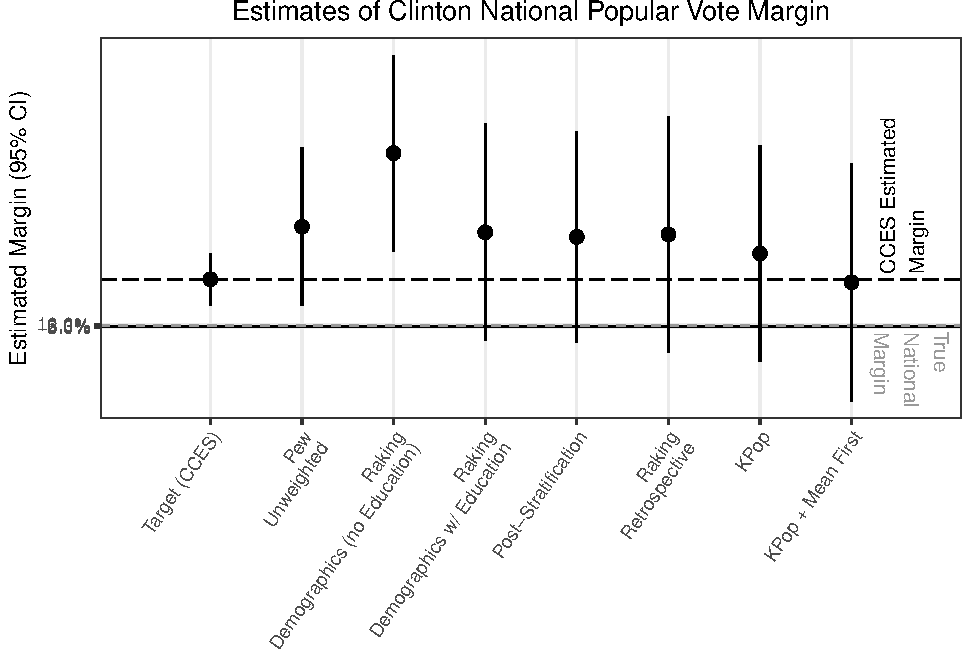
\includegraphics{application_clean_files/figure-latex/plot_results-1.pdf}

\begin{Shaded}
\begin{Highlighting}[]
\KeywordTok{ggsave}\NormalTok{(}\StringTok{"./plots/weighted_pew_results.pdf"}\NormalTok{, }\DataTypeTok{width =} \DecValTok{6}\NormalTok{, }\DataTypeTok{height =} \DecValTok{4}\NormalTok{)}
\end{Highlighting}
\end{Shaded}

Note from \texttt{survey} package:

The design effect compares the variance of a mean or total to the
variance from a study of the same size using simple random sampling
without replacement. Note that the design effect will be incorrect if
the weights have been rescaled so that they are not reciprocals of
sampling probabilities. To obtain an estimate of the design effect
comparing to simple random sampling with replacement, which does not
have this requirement, use \texttt{deff="replace"}. This
with-replacement design effect is the square of Kish's ``deft''.

\begin{Shaded}
\begin{Highlighting}[]
\KeywordTok{lapply}\NormalTok{(}\KeywordTok{list}\NormalTok{(rake_demos_noeduc, rake_demos_weduc, post_stratification, rake_retrospective, kpop, kpop_mf), }
       \ControlFlowTok{function}\NormalTok{(x) \{}
         \KeywordTok{svymean}\NormalTok{(}\OperatorTok{~}\NormalTok{recode_vote_}\DecValTok{2016}\NormalTok{, x, }\DataTypeTok{deff =} \StringTok{"replace"}\NormalTok{)}
\NormalTok{       \})}
\end{Highlighting}
\end{Shaded}

\begin{verbatim}
## [[1]]
##                                 mean        SE   DEff
## recode_vote_2016Democrat   0.5152342 0.0137716 1.5741
## recode_vote_2016Other      0.0610503 0.0068547 1.6992
## recode_vote_2016Republican 0.4237155 0.0135460 1.5578
## 
## [[2]]
##                                mean       SE   DEff
## recode_vote_2016Democrat   0.492440 0.015599 2.0182
## recode_vote_2016Other      0.064585 0.010645 3.8881
## recode_vote_2016Republican 0.442974 0.015397 1.9917
## 
## [[3]]
##                                 mean        SE   DEff
## recode_vote_2016Democrat   0.4951602 0.0146016 1.7681
## recode_vote_2016Other      0.0570701 0.0064833 1.6192
## recode_vote_2016Republican 0.4477697 0.0147349 1.8202
## 
## [[4]]
##                                 mean        SE   DEff
## recode_vote_2016Democrat   0.4955713 0.0162761 2.1968
## recode_vote_2016Other      0.0575692 0.0077328 2.2847
## recode_vote_2016Republican 0.4468595 0.0165905 2.3084
## 
## [[5]]
##                                 mean        SE   DEff
## recode_vote_2016Democrat   0.4911832 0.0149371 1.8507
## recode_vote_2016Other      0.0562514 0.0062328 1.5170
## recode_vote_2016Republican 0.4525654 0.0149954 1.8815
## 
## [[6]]
##                                mean       SE   DEff
## recode_vote_2016Democrat   0.482228 0.016914 2.3751
## recode_vote_2016Other      0.058803 0.010303 3.9758
## recode_vote_2016Republican 0.458969 0.016838 2.3668
\end{verbatim}

\hypertarget{weights}{%
\subsection{Weights}\label{weights}}

Looking at the average weight in margins.

\begin{Shaded}
\begin{Highlighting}[]
\KeywordTok{load}\NormalTok{(}\StringTok{"cleaned data/Full SVD/weights_wPid_full.Rdata"}\NormalTok{)}
\CommentTok{#optimal choice w pid: no mf = 0.5, mf = 2}
\NormalTok{weights <-}\StringTok{ }\NormalTok{pew }\OperatorTok\StringTok{ }\KeywordTok{select}\NormalTok{(recode_age_bucket,}
\NormalTok{                          recode_age_3way,}
\NormalTok{                          recode_female,}
\NormalTok{                          recode_race,}
\NormalTok{                          recode_region,}
\NormalTok{                          recode_educ,}
\NormalTok{                          recode_educ_3way,}
\NormalTok{                          recode_pid_3way,}
\NormalTok{                          recode_race_educ_reg)  }\OperatorTok
\StringTok{    }\KeywordTok{mutate}\NormalTok{(}\DataTypeTok{rake_demos_noeduc_wt =} \KeywordTok{weights}\NormalTok{(rake_demos_noeduc)}\OperatorTok{/}
\StringTok{                                 }\KeywordTok{mean}\NormalTok{(}\KeywordTok{weights}\NormalTok{(rake_demos_noeduc)),}
           \DataTypeTok{rake_demos_weduc_wt =} \KeywordTok{weights}\NormalTok{(rake_demos_weduc)}\OperatorTok{/}
\StringTok{                                 }\KeywordTok{mean}\NormalTok{(}\KeywordTok{weights}\NormalTok{(rake_demos_weduc)),}
           \DataTypeTok{post_stratification_wt =} \KeywordTok{weights}\NormalTok{(post_stratification)}\OperatorTok{/}
\StringTok{                                 }\KeywordTok{mean}\NormalTok{(}\KeywordTok{weights}\NormalTok{(post_stratification)),}
           \DataTypeTok{rake_retrospective_wt =} \KeywordTok{weights}\NormalTok{(rake_retrospective)}\OperatorTok{/}
\StringTok{                                 }\KeywordTok{mean}\NormalTok{(}\KeywordTok{weights}\NormalTok{(rake_retrospective)),}
           \DataTypeTok{k_wt =}\NormalTok{ wts_wPid}\OperatorTok{$}\NormalTok{wtkbal_b}\FloatTok{.5}\NormalTok{x,}
           \DataTypeTok{k_mf_wt =}\NormalTok{ wts_wPid}\OperatorTok{$}\NormalTok{wtkbal_mf_b2x)}

\CommentTok{#just checking everything is internally consistent}
\CommentTok{#sum(weights$rake_demos_noeduc_wt != wts_wPid$wt1_pid)}

\NormalTok{age <-}\StringTok{ }\NormalTok{weights }\OperatorTok\StringTok{ }
\StringTok{    }\KeywordTok{group_by}\NormalTok{(recode_age_bucket) }\OperatorTok\StringTok{ }
\StringTok{    }\KeywordTok{summarise}\NormalTok{(}\DataTypeTok{mu_1 =} \KeywordTok{mean}\NormalTok{(rake_demos_noeduc_wt),}
              \DataTypeTok{mu_2 =} \KeywordTok{mean}\NormalTok{(rake_demos_weduc_wt),}
              \DataTypeTok{mu_3 =} \KeywordTok{mean}\NormalTok{(post_stratification_wt),}
              \DataTypeTok{mu_4 =} \KeywordTok{mean}\NormalTok{(rake_retrospective_wt),}
              \DataTypeTok{mu_kpop =} \KeywordTok{mean}\NormalTok{(k_wt),}
              \DataTypeTok{mu_kpop_mf =} \KeywordTok{mean}\NormalTok{(k_mf_wt)) }\OperatorTok\StringTok{ }\KeywordTok{ungroup}\NormalTok{()}

\NormalTok{female <-}\StringTok{ }\NormalTok{weights }\OperatorTok\StringTok{ }
\StringTok{    }\KeywordTok{group_by}\NormalTok{(recode_female) }\OperatorTok\StringTok{ }
\StringTok{    }\KeywordTok{summarise}\NormalTok{(}\DataTypeTok{mu_1 =} \KeywordTok{mean}\NormalTok{(rake_demos_noeduc_wt),}
              \DataTypeTok{mu_2 =} \KeywordTok{mean}\NormalTok{(rake_demos_weduc_wt),}
              \DataTypeTok{mu_3 =} \KeywordTok{mean}\NormalTok{(post_stratification_wt),}
              \DataTypeTok{mu_4 =} \KeywordTok{mean}\NormalTok{(rake_retrospective_wt),}
              \DataTypeTok{mu_kpop =} \KeywordTok{mean}\NormalTok{(k_wt),}
              \DataTypeTok{mu_kpop_mf =} \KeywordTok{mean}\NormalTok{(k_mf_wt)) }\OperatorTok\StringTok{ }\KeywordTok{ungroup}\NormalTok{()}

\NormalTok{race <-}\StringTok{ }\NormalTok{weights }\OperatorTok\StringTok{ }
\StringTok{    }\KeywordTok{group_by}\NormalTok{(recode_race) }\OperatorTok\StringTok{ }
\StringTok{    }\KeywordTok{summarise}\NormalTok{(}\DataTypeTok{mu_1 =} \KeywordTok{mean}\NormalTok{(rake_demos_noeduc_wt),}
              \DataTypeTok{mu_2 =} \KeywordTok{mean}\NormalTok{(rake_demos_weduc_wt),}
              \DataTypeTok{mu_3 =} \KeywordTok{mean}\NormalTok{(post_stratification_wt),}
              \DataTypeTok{mu_4 =} \KeywordTok{mean}\NormalTok{(rake_retrospective_wt),}
              \DataTypeTok{mu_kpop =} \KeywordTok{mean}\NormalTok{(k_wt),}
              \DataTypeTok{mu_kpop_mf =} \KeywordTok{mean}\NormalTok{(k_mf_wt)) }\OperatorTok\StringTok{ }\KeywordTok{ungroup}\NormalTok{()}

\NormalTok{region <-}\StringTok{ }\NormalTok{weights }\OperatorTok\StringTok{ }
\StringTok{    }\KeywordTok{group_by}\NormalTok{(recode_region) }\OperatorTok
\StringTok{    }\KeywordTok{summarise}\NormalTok{(}\DataTypeTok{mu_1 =} \KeywordTok{mean}\NormalTok{(rake_demos_noeduc_wt),}
              \DataTypeTok{mu_2 =} \KeywordTok{mean}\NormalTok{(rake_demos_weduc_wt),}
              \DataTypeTok{mu_3 =} \KeywordTok{mean}\NormalTok{(post_stratification_wt),}
              \DataTypeTok{mu_4 =} \KeywordTok{mean}\NormalTok{(rake_retrospective_wt),}
              \DataTypeTok{mu_kpop =} \KeywordTok{mean}\NormalTok{(k_wt),}
              \DataTypeTok{mu_kpop_mf =} \KeywordTok{mean}\NormalTok{(k_mf_wt)) }\OperatorTok\StringTok{ }\KeywordTok{ungroup}\NormalTok{()}

\NormalTok{education <-}\StringTok{ }\NormalTok{weights }\OperatorTok\StringTok{ }
\StringTok{    }\KeywordTok{group_by}\NormalTok{(recode_educ) }\OperatorTok\StringTok{ }
\StringTok{    }\KeywordTok{summarise}\NormalTok{(}\DataTypeTok{mu_1 =} \KeywordTok{mean}\NormalTok{(rake_demos_noeduc_wt),}
              \DataTypeTok{mu_2 =} \KeywordTok{mean}\NormalTok{(rake_demos_weduc_wt),}
              \DataTypeTok{mu_3 =} \KeywordTok{mean}\NormalTok{(post_stratification_wt),}
              \DataTypeTok{mu_4 =} \KeywordTok{mean}\NormalTok{(rake_retrospective_wt),}
              \DataTypeTok{mu_kpop =} \KeywordTok{mean}\NormalTok{(k_wt),}
              \DataTypeTok{mu_kpop_mf =} \KeywordTok{mean}\NormalTok{(k_mf_wt)) }\OperatorTok\StringTok{ }\KeywordTok{ungroup}\NormalTok{()}

\NormalTok{pid <-}\StringTok{ }\NormalTok{weights }\OperatorTok\StringTok{ }
\StringTok{    }\KeywordTok{group_by}\NormalTok{(recode_pid_3way) }\OperatorTok\StringTok{ }
\StringTok{    }\KeywordTok{summarise}\NormalTok{(}\DataTypeTok{mu_1 =} \KeywordTok{mean}\NormalTok{(rake_demos_noeduc_wt),}
              \DataTypeTok{mu_2 =} \KeywordTok{mean}\NormalTok{(rake_demos_weduc_wt),}
              \DataTypeTok{mu_3 =} \KeywordTok{mean}\NormalTok{(post_stratification_wt),}
              \DataTypeTok{mu_4 =} \KeywordTok{mean}\NormalTok{(rake_retrospective_wt),}
              \DataTypeTok{mu_kpop =} \KeywordTok{mean}\NormalTok{(k_wt),}
              \DataTypeTok{mu_kpop_mf =} \KeywordTok{mean}\NormalTok{(k_mf_wt)) }\OperatorTok\StringTok{ }\KeywordTok{ungroup}\NormalTok{()}


\KeywordTok{colnames}\NormalTok{(age) <-}\StringTok{ }\KeywordTok{c}\NormalTok{(}\StringTok{"Variable"}\NormalTok{, }\KeywordTok{colnames}\NormalTok{(age)[}\OperatorTok{-}\DecValTok{1}\NormalTok{])}
\KeywordTok{colnames}\NormalTok{(female)<-}\StringTok{ }\KeywordTok{c}\NormalTok{(}\StringTok{"Variable"}\NormalTok{, }\KeywordTok{colnames}\NormalTok{(female)[}\OperatorTok{-}\DecValTok{1}\NormalTok{])}
\KeywordTok{colnames}\NormalTok{(race)<-}\StringTok{ }\KeywordTok{c}\NormalTok{(}\StringTok{"Variable"}\NormalTok{, }\KeywordTok{colnames}\NormalTok{(race)[}\OperatorTok{-}\DecValTok{1}\NormalTok{])}
\KeywordTok{colnames}\NormalTok{(region) <-}\StringTok{ }\KeywordTok{c}\NormalTok{(}\StringTok{"Variable"}\NormalTok{, }\KeywordTok{colnames}\NormalTok{(region)[}\OperatorTok{-}\DecValTok{1}\NormalTok{])}
\KeywordTok{colnames}\NormalTok{(education) <-}\StringTok{ }\KeywordTok{c}\NormalTok{(}\StringTok{"Variable"}\NormalTok{, }\KeywordTok{colnames}\NormalTok{(education)[}\OperatorTok{-}\DecValTok{1}\NormalTok{])}
\KeywordTok{colnames}\NormalTok{(pid) <-}\StringTok{ }\KeywordTok{c}\NormalTok{(}\StringTok{"Variable"}\NormalTok{, }\KeywordTok{colnames}\NormalTok{(pid)[}\OperatorTok{-}\DecValTok{1}\NormalTok{])}

\NormalTok{weights_summary <-}\StringTok{ }\KeywordTok{rbind}\NormalTok{(age, female, race, region, education, pid) }
\end{Highlighting}
\end{Shaded}

\begin{table}[t]

\caption{\label{tab:weights_print}Mean weights of important demographics under different weighting models .}
\centering
\begin{threeparttable}
\begin{tabular}{>{\raggedright\arraybackslash}p{1.45in}>{\raggedleft\arraybackslash}p{0.45in}>{\raggedleft\arraybackslash}p{0.45in}>{\raggedleft\arraybackslash}p{0.45in}>{\raggedleft\arraybackslash}p{0.45in}>{\raggedleft\arraybackslash}p{0.45in}>{\raggedleft\arraybackslash}p{0.45in}}
\toprule
 & \belowbaseline[0ex]{\rotatebox{90}{\parbox{1.1in}{\raggedright{Raking \\Demographics without Education }}}} & \belowbaseline[0ex]{\rotatebox{90}{\parbox{1.1in}{\raggedright{Raking \\Demographics with Education }}}} & \belowbaseline[0ex]{\rotatebox{90}{\parbox{1.1in}{\raggedright{Post-Stratification}}}} & \belowbaseline[0ex]{\rotatebox{90}{\parbox{1.1in}{\raggedright{Raking Retrospective}}}} & \belowbaseline[0ex]{\rotatebox{90}{\parbox{1.1in}{\raggedright{KPop}}}} & \belowbaseline[0ex]{\rotatebox{90}{\parbox{1.1in}{\raggedright{KPop Mean First}}}}\\
\midrule
\addlinespace[0.5em]
\multicolumn{7}{l}{\textbf{4-way Age Bucket}}\\
\hspace{1em}18 to 35 & 0.795 & 0.795 & 0.809 & 0.795 & 0.787 & 0.795\\
\hspace{1em}36 to 50 & 0.692 & 0.692 & 0.818 & 0.692 & 0.722 & 0.692\\
\hspace{1em}51 to 64 & 1.378 & 1.378 & 1.415 & 1.378 & 1.406 & 1.378\\
\hspace{1em}65+ & 5.183 & 5.183 & 3.117 & 5.183 & 4.732 & 5.183\\
\addlinespace[0.5em]
\multicolumn{7}{l}{\textbf{Gender}}\\
\hspace{1em}Female & 1.076 & 1.076 & 1.075 & 1.076 & 1.075 & 1.076\\
\hspace{1em}Male & 0.932 & 0.932 & 0.933 & 0.932 & 0.933 & 0.932\\
\addlinespace[0.5em]
\multicolumn{7}{l}{\textbf{Race/Ethnicity}}\\
\hspace{1em}Black & 1.326 & 1.326 & 1.293 & 1.515 & 1.318 & 1.326\\
\hspace{1em}Hispanic & 0.857 & 0.857 & 0.815 & 0.857 & 0.770 & 0.857\\
\hspace{1em}Other & 0.955 & 0.955 & 0.911 & 0.955 & 0.865 & 0.955\\
\hspace{1em}White & 0.981 & 0.981 & 0.993 & 0.959 & 0.999 & 0.981\\
\addlinespace[0.5em]
\multicolumn{7}{l}{\textbf{Region}}\\
\hspace{1em}Midwest & 1.052 & 1.052 & 1.043 & 1.110 & 1.061 & 1.052\\
\hspace{1em}Northeast & 1.081 & 1.081 & 1.057 & 1.081 & 1.071 & 1.081\\
\hspace{1em}South & 0.935 & 0.935 & 0.972 & 0.916 & 0.949 & 0.935\\
\hspace{1em}West & 0.994 & 0.994 & 0.956 & 0.965 & 0.966 & 0.994\\
\addlinespace[0.5em]
\multicolumn{7}{l}{\textbf{Education Level}}\\
\hspace{1em}No HS & 1.000 & 3.823 & 1.320 & 2.030 & 1.062 & 3.823\\
\hspace{1em}High school & 1.091 & 1.553 & 1.463 & 1.492 & 1.586 & 1.553\\
\hspace{1em}Some college & 1.059 & 1.374 & 1.467 & 1.374 & 1.457 & 1.374\\
\hspace{1em}2-year & 0.937 & 0.936 & 0.840 & 1.029 & 0.963 & 0.936\\
\hspace{1em}4-year & 0.915 & 0.653 & 0.777 & 0.707 & 0.711 & 0.653\\
\hspace{1em}Post-grad & 1.017 & 0.474 & 0.575 & 0.556 & 0.516 & 0.474\\
\addlinespace[0.5em]
\multicolumn{7}{l}{\textbf{Party Identification}}\\
\hspace{1em}Dem & 1.105 & 1.105 & 1.119 & 1.105 & 1.093 & 1.105\\
\hspace{1em}Ind & 0.922 & 0.922 & 0.924 & 0.922 & 0.933 & 0.922\\
\hspace{1em}Rep & 0.971 & 0.971 & 0.954 & 0.971 & 0.973 & 0.971\\
\bottomrule
\end{tabular}
\begin{tablenotes}
\item \textit{Note: } 
\item Cells present the average weight used to reweight the Pew sample to the CCES target population in each variable level.
\end{tablenotes}
\end{threeparttable}
\end{table}


\end{document}
